\documentclass[11pt,a4paper,twoside]{report}
\usepackage[utf8]{inputenc}
\usepackage[portuguese]{babel}
\usepackage[T1]{fontenc}
\usepackage{fancyhdr}
\usepackage{amsmath}
\usepackage{amsfonts}
\usepackage{amssymb}
\usepackage{makeidx}
\usepackage{graphicx}
\usepackage{lmodern}
\usepackage{wrapfig}
\usepackage{color}
\usepackage{float}
%\usepackage{fourier}
\usepackage[left=2cm,right=2cm,top=2cm,bottom=2cm]{geometry}
\author{Bartolomeu J. Ubisse}
\pagestyle{fancy}
\renewcommand{\headrulewidth}{0pt}
\renewcommand{\footrulewidth}{1pt}
\fancyfoot[L]{ | UEM - 2017}
\fancyfoot[c]{}
\fancyfoot[r]{\thepage}
\begin{document}


\begin{figure}[htb]

\centering

\includegraphics[scale=1]{UEM-logotipo}
\end{figure}
\centering
{ \Large Universidade Eduardo Mondlane}\\[0.3cm] 
\large Faculdade de Ci\^encias\\[0.2cm]
 \large Departamento de F\'isica\\[0.5cm]

%\textsc{Electr\^onica B\'asica} \\[1cm]
\begin{flushleft}
\tt Teste 2 -Laboral - E. Anal\'ogica - Corre\c c\~ao \\
\hrulefill
\end{flushleft}

\begin{enumerate}
\item i) Equivalente Thevenin
\begin{figure}[H]
\centering
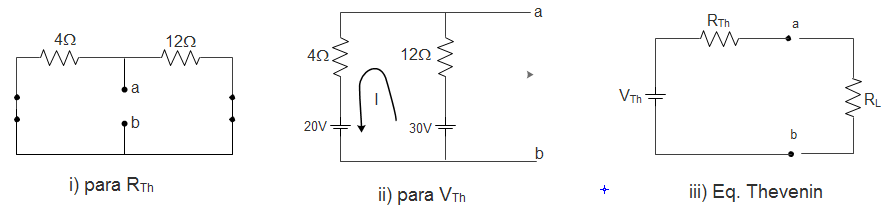
\includegraphics[scale=0.6]{Thevenin}
\caption{}
\label{f2}
\end{figure}
\textbf{Da fig.\ref{f2}} - i: $R_{Th}=\frac{12\times4}{12+4}\Omega=3\Omega$\\
\vspace{0.3cm}

\textbf{Da fig.\ref{f2}} - ii:\\ $(30-20)$V$=I\times(12+4)\Omega \longrightarrow I=0.625$A\\
\vspace{0.3cm}
$V_{Th}=30$ V $-I\times 12\Omega \longrightarrow V_{Th}=22.5$V\\
\vspace{0.3cm}
\textbf{Da fig.\ref{f2}} - iii: $V_{RL}=\frac{R_L}{R_L+R_{Th}}\times V_{Th}=18V$\\

\vspace{0.5cm}
ii) Teorema de superposi\c c\~ao:

\noindent
\begin{minipage}[c]{6.5cm}
\begin{figure}[H]
\centering
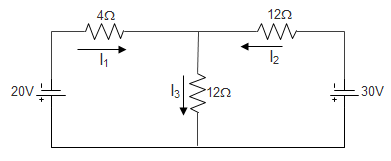
\includegraphics[scale=0.8]{superp1}
\caption{}
\label{f3}
\end{figure}
\end{minipage}\hfill
\begin{minipage}[c]{6.5cm}
{Repare que para determinar a queda de tens\~ao no resistor $R_L$, precisa-se de $I_3$.\\
\'E importante comparar os sentidos da corrente atrav\'es do $R_L$ dos passos parciais com o do sentido da fig.\ref{f3}.}
\end{minipage}

\textbf{$1^0$ Passo:}
\noindent
\begin{minipage}[c]{6.5cm}
\begin{figure}[H]
\centering
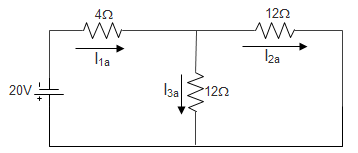
\includegraphics[scale=0.8]{superp1a}
\caption{}
\label{f4}
\end{figure}
\end{minipage}\hfill
\begin{minipage}[c]{6.5cm}
{$I_{1a}=\frac{20V}{\left[ \frac{12\times12}{12+12}+4\right] \Omega}=2$A\\

$I_{3a}=\frac{12\Omega}{\left[12+12\right] \Omega}\times2A=1$A
}
\end{minipage}

\textbf{$2^0$ Passo:}
\noindent
\begin{minipage}[c]{6.5cm}
\begin{figure}[H]
\centering
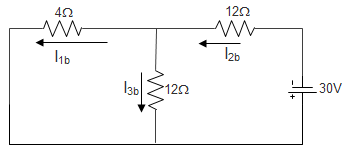
\includegraphics[scale=0.8]{superp1b}
\caption{}
\label{f5}
\end{figure}
\end{minipage}\hfill
\begin{minipage}[c]{6.5cm}
{$I_{2b}=\frac{30V}{\left[ \frac{12\times4}{12+4}+12\right] \Omega}=2$A\\

$I_{3b}=\frac{4\Omega}{\left[4+12\right] \Omega}\times2$A$=0.5$A
}
\end{minipage}

Ent\~ao:

$I_3=I_{3a}+I_{3b}=1.5$A\\

$V_{RL}=I_3\times R_L \longrightarrow V_{RL}=1.5A\times 12\Omega=18V$


\item A energia de banda proibida \'e a energia de separa\c c\~ao entre o n\'ivel mais baixo da banda de condu\c c\~ao e o n\'ivel mais alto da banda de val\^encia. Visto que os portadores de carga dever\~ao transitar da banda de val\^encia para a banda de condu\c c\~ao, ent\~ao, essa \'e a m\'inima energia que os portadores de carga devem ter com vista a transitarem  at\'e a banda de condu\c c\~ao. $E_{g-Isoladores}>E_{g-S/condutores}>E_{g-Condutores}$.

\item Para que se obtenha um material de sil\'icio de tipo $P$, \'e necess\'ario que dope o material intr\'insico com \'atomos do grupo - III da tabela peri\'odica, como por exemplo, o borro. Ap\'os a dopagem com \'atomos trivalentes, o material de sil\'icio fica com excesso de lacunas, isto \'e, os portadores maiorit\'arios s\~ao lacunas e, uma vez que a impureza recebe um electr\~ao da rede do sil\'icio, ent\~ao ela torna-se um i\~ao negativo.

\item Quando dois materiais extr\'insecos um do tipo $P$ e outro do tipo $N$ s\~ao unidos, ocorre uma difus\~ao de portadores de cargas e em fun\c c\~ao disso h\'a uma corrente de difus\~ao ($\vec J_{dif}$). Durante o processo da difus\~ao algumas cargas (positivas do lado $N$ e negativas do lado $P$) junto \'a inteface deixam de ser neutralizadas e d\~ao origem a um campo el\'ectrico cujo sentido \'e do lado $N$ para o lado $P$ e, por meio disso tem-se uma corrente no mesmo sentido denominado corrente de deriva ($\vec J_{der}$). Quando essas duas correntes se igualam ent\~ao nenhum portador de carga passa atrav\'es da jun\c c\~ao e a mesma comporta-se como um dipolo el\'ectrico e com uma diferen\c ca de potencial que, para o caso de sil\'icio varia de 6V a 8V.  


\item \'E necess\'ario que o cursor do mult\'imetro esteja na posi\c c\~ao do d\'iodo e em seguida polarize-se directamente o d\'iodo. Se o d\'iodo n\~ao tiver defeito, o multimetro vai registar um valor na ordem de 500 a 800 mV e, quando se inverter a polariza\c c\~ao, ele vai indicar 1 (valor que indica mesmo quando n\~ao estiver ligado a nenhum dispositivo). Em caso de defeito, o mult\'imetro ou vai registar um valor muito baixo acompanhado de um som (quando estiver em curto) ou vai indicar 1 (no caso de o d\'iodo estiver em aberto). De notar que em caso de curto, o mult\'imetro regista esse valor tanto na poriza\c c\~ao directa assim como na inversa.

\item $V_r=\frac{V_p}{2fRC}$, logo: $C_{V_r=0.2V}=0.2mF$ e $C_{V_r=0.5V}=83\mu F$. O capacitor de $0.2mF$ \'e melhor porque permite ter um sinal com ondula\c c\~ao relativamente menor.



\item Tens\~oes m\'axima e m\'inima: 

\begin{figure}[H]
\centering
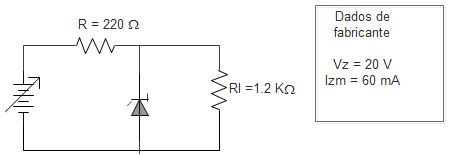
\includegraphics[scale=1]{cZener}
\caption{Circu\'ito regulador}
\label{f1}
\end{figure}

$V_{min}=\frac{R_L+R}{R_L}\times V_L \longrightarrow V_{min}=\frac{1200+220}{1200}\times 20=23.67 $V\\
\vspace{0.3cm}
$I_L=\frac{V_L}{R_L}\longrightarrow I_L=\frac{20V}{1200\Omega}=16.67mA$\\
\vspace{0.3cm}
$I_{RM}=I_{ZM}+I_L \longrightarrow I_{RM}=60 mA+16.67mA=76.67mA$\\
\vspace{0.3cm}
$V_{max}=I_{ZM}\times V_Z=36.87V$\\

\begin{enumerate}
\item[a)]

O esbo\c co \'e: 
\begin{figure}[H]
\centering
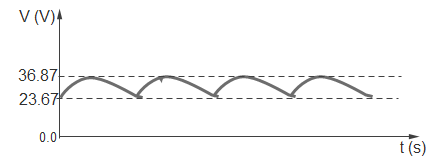
\includegraphics[scale=1]{ripple}
\caption{}
\label{f1}
\end{figure}
\end{enumerate}


\end{enumerate}



\Huge FIM


\end{document}